Los diagramas de bloques de los Capítulos \ref{chapter:deteccion ruido} y \ref{chapter:modulacion pasabanda} (Figuras \ref{fig:deteccion ruido} y \ref{fig:deteccion canal ruido}) vienen arrastrando una caja llamada ``Sincronismo'', conectada con una flecha punteada, que nunca se abre -- se supuso siempre, como dice explícitamente el texto que acompaña a la Figura \ref{fig:deteccion ruido}, que ``conocemos el momento exacto donde muestrear la onda recibida'', sin decir cómo se logra eso en la práctica. Este capítulo abre esa caja.

\subsection*{El problema del sincronismo}

Repasemos qué venimos suponiendo, sin decirlo, desde hace varios capítulos. El detector coherente de la Sección \ref{sec:deteccion coherente} multiplica la señal recibida por $2\cos(2\pi f_c t)$ y $-2\sin(2\pi f_c t)$ -- osciladores locales de frecuencia \emph{exactamente} $f_c$ y fase \emph{exactamente} alineada con el oscilador que generó la portadora en el transmisor. Y el detector de la Figura \ref{fig:deteccion ruido} muestrea la salida del filtro de recepción en el instante $kT_s$ -- suponiendo que \emph{conocemos} ese instante con precisión. Ninguna de las dos cosas es gratis: el transmisor y el receptor son dos dispositivos físicamente separados, cada uno con su propio oscilador de referencia (un cristal de cuarzo, típicamente) y su propio reloj de muestreo, sin ningún cable en común que los sincronice.

Aunque los osciladores de transmisor y receptor estén diseñados para la misma frecuencia nominal $f_c$, ningún cristal real oscila a una frecuencia exacta -- hay una tolerancia de fabricación (típicamente unas pocas partes por millón). El oscilador local del receptor tiene entonces una frecuencia $f_c+\Delta f$, con $\Delta f$ un \emph{offset de frecuencia de portadora} (\emph{Carrier Frequency Offset}, CFO) desconocido pero acotado, y una fase inicial arbitraria. Lo mismo ocurre, de forma independiente, con el reloj que define los instantes de muestreo $kT_s$: puede estar corrido en fase, o incluso avanzar a una velocidad ligeramente distinta a $f_s$. Sin corregir estos desajustes, ni la fase de la constelación ni el instante de muestreo son los que el resto del texto supone.

El problema del sincronismo tiene, entonces, tres capas, que conviene distinguir porque se resuelven con mecanismos distintos y en un orden lógico:
\begin{enumerate}
    \item \textbf{Sincronización de portadora}: estimar y corregir el CFO y la fase del oscilador local, para que la demodulación coherente (Sección \ref{sec:deteccion coherente}) entregue realmente $x_i(t)\approx\sum a_k p(t-kT_s)$ y no una versión rotada, con energía filtrándose entre las componentes en fase y cuadratura.
    \item \textbf{Temporización de símbolo}: estimar el instante correcto de muestreo $kT_s$, para que la muestra tomada corresponda al máximo del pulso (o, más generalmente, al punto de ISI nula que garantiza el pulso de Nyquist, Sección \ref{sec:nyquist no ideal}).
    \item \textbf{Sincronización de trama}: una vez enganchados portadora y reloj de símbolo, saber \emph{dónde empieza el mensaje} dentro del flujo continuo de símbolos -- y, como veremos, resolver de paso una ambigüedad de fase que las dos capas anteriores dejan sin resolver.
\end{enumerate}
Las primeras dos capas comparten una misma herramienta matemática -- un \emph{lazo de enganche de fase} (\emph{Phase-Locked Loop}, PLL) -- aplicada a dos variables físicas distintas (fase de portadora, fase de reloj de símbolo). Conviene entonces derivar el lazo genérico una sola vez, y después particularizarlo dos veces.

\subsection*{El lazo de enganche de fase (PLL)}\label{sec:pll generico}

Un PLL es un sistema realimentado que ajusta la fase de un oscilador local hasta que coincide con la de una referencia entrante. Tres bloques lo componen (Figura \ref{fig:pll generico}):
\begin{itemize}
    \item Un \emph{detector de fase}, que compara la fase $\theta_{in}(t)$ de la señal entrante con la fase $\theta_{vco}(t)$ del oscilador local, y produce una señal de error $e(t)$ proporcional (para error chico) a la diferencia: $e(t) \approx K_d\,\big(\theta_{in}(t)-\theta_{vco}(t)\big)$, con $K_d$ la ganancia del detector.
    \item Un \emph{filtro de lazo}, que suaviza $e(t)$ -- en su versión más simple, una ganancia pura, que es la que consideramos aquí (\emph{lazo de primer orden}).
    \item Un \emph{oscilador controlado por tensión} (VCO), cuya frecuencia instantánea es proporcional a la tensión de control $v(t)$ que recibe: $\displaystyle\frac{d\theta_{vco}}{dt} = K_{vco}\, v(t)$, con $K_{vco}$ la sensibilidad del VCO. Es decir, el VCO \emph{integra} su entrada para producir una fase.
\end{itemize}

\begin{figure}
    \begin{center}
    \begin{blockdiagram}
        \node [etiqueta] (inicio) {$\theta_{in}(t)$};
        \node [operator, right=1.3cm of inicio] (sum) {$+$};
        \node [block, right=2.6cm of sum, align=center] (fd) {Detector\\de fase};
        \node [block, right=3.4cm of fd, align=center] (vco) {VCO\\[2pt]\footnotesize$\frac{d\theta_{vco}}{dt}=K_{vco}v(t)$};
        \node [etiqueta, right=1.8cm of vco] (salida) {$\theta_{vco}(t)$};
        \draw [->] (inicio) -- (sum);
        \draw [->] (sum) -- node[midway,above] {\footnotesize $\theta_e(t)$} (fd);
        \draw [->] (fd) -- node[midway,above] {\footnotesize $e(t)\approx K_d\theta_e(t)$} (vco);
        \draw [->] (vco) -- (salida);
        \draw [->] (vco.south) -- ++(0,-1.2) -| node[near start, below, xshift=-3.2cm]{\footnotesize $-\theta_{vco}(t)$} (sum.south);
    \end{blockdiagram}
    \end{center}
    \caption{Lazo de enganche de fase (PLL) genérico, de primer orden: el detector de fase compara la referencia entrante con la realimentación del propio VCO, y la diferencia corrige la frecuencia de este último hasta anular el error.}\label{fig:pll generico}
\end{figure}

Definamos el error de fase $\theta_e(t) := \theta_{in}(t) - \theta_{vco}(t)$. Combinando las tres relaciones del lazo se obtiene su comportamiento:

\begin{proposicion}[Dinámica del lazo de primer orden]\label{prop:pll dinamica}
Con $K:=K_{vco}K_d$ (la \emph{ganancia de lazo}), el error de fase satisface
\begin{equation}\label{eq:pll edo}
    \frac{d\theta_e}{dt} + K\,\theta_e(t) = \frac{d\theta_{in}}{dt}.
\end{equation}
En particular:
\begin{enumerate}
    \item[(a)] Ante un salto de fase puro (la fase entrante salta $\Delta\theta$ en $t=0$ y luego permanece a frecuencia nominal, $d\theta_{in}/dt=0$ para $t>0$), el error decae exponencialmente,
    \begin{equation*}
        \theta_e(t) = \theta_e(0)\,\e^{-Kt},
    \end{equation*}
    con constante de tiempo $1/K$: el lazo \emph{engancha}.
    \item[(b)] Ante un offset de frecuencia constante $\Delta f$ (la fase entrante es $\theta_{in}(t)=2\pi\Delta f\,t+\theta_0$), el error de fase converge a un valor residual constante,
    \begin{equation}\label{eq:pll error regimen}
        \theta_{e,\infty} = \frac{2\pi\Delta f}{K}.
    \end{equation}
\end{enumerate}
\end{proposicion}
\begin{proof}
Derivando $\theta_e$ y sustituyendo las dos relaciones del lazo ($v(t)=e(t)\approx K_d\theta_e(t)$ para el filtro de lazo sin filtrado adicional, y $d\theta_{vco}/dt=K_{vco}v(t)$ para el VCO):
\begin{equation*}
    \frac{d\theta_e}{dt} = \frac{d\theta_{in}}{dt} - \frac{d\theta_{vco}}{dt} = \frac{d\theta_{in}}{dt} - K_{vco}K_d\,\theta_e(t),
\end{equation*}
que es \eqref{eq:pll edo}. Para (a), con $d\theta_{in}/dt=0$, la ecuación homogénea $\dot\theta_e=-K\theta_e$ tiene solución $\theta_e(t)=\theta_e(0)\e^{-Kt}$. Para (b), en régimen permanente ($\dot\theta_e=0$), \eqref{eq:pll edo} da directamente $K\theta_{e,\infty}=2\pi\Delta f$.
\end{proof}

Cuanto mayor la ganancia $K$, más rápida la adquisición en (a) y menor el error residual en (b) -- pero (aunque no lo desarrollamos aquí) también ensancha la banda de ruido que el lazo deja pasar: hay un compromiso entre velocidad de adquisición/error residual y inmunidad al ruido en la elección de $K$.

Con este comportamiento genérico -- adquisición exponencial, con constante de tiempo $1/K$, y error residual ante un offset de frecuencia -- vamos a reencontrarnos dos veces: primero enganchando la fase de la portadora, después enganchando la fase del reloj de muestreo. En ambos casos la ecuación \eqref{eq:pll edo} es la misma; lo que cambia es qué señal física hace de $\theta_{in}(t)$ y cómo se construye el detector de fase.

\subsection*{Sincronización de portadora: el lazo de Costas}

Apliquemos el PLL genérico al problema de la Sección \ref{sec:deteccion coherente}. Sea, para BPSK, $x_c(t) = \sum_k a_k\, p(t-kT_s)\cos(2\pi f_c t+\theta)$, con $a_k\in\{-A,A\}$ y $\theta$ la fase (desconocida) del oscilador transmisor. El receptor genera localmente $2\cos(2\pi f_c t+\theta_{vco})$ y $-2\sin(2\pi f_c t+\theta_{vco})$, con $\theta_{vco}$ la fase de su propio VCO -- la estimación actual de $\theta$, y $\theta_e:=\theta-\theta_{vco}$ el error de fase que queremos anular.

\begin{proposicion}[Señal de error del lazo de Costas]\label{prop:costas}
Con $m(t):=\sum_k a_k\, p(t-kT_s)$, las salidas de los mezcladores del receptor son
\begin{equation}\label{eq:xi xq con error de fase}
    x_i(t) \approx m(t)\cos\theta_e, \qquad\qquad x_q(t) \approx m(t)\sin\theta_e,
\end{equation}
y su producto resulta, para $\theta_e$ chico,
\begin{equation}\label{eq:error costas}
    e(t) := x_i(t)\,x_q(t) \approx \frac{m(t)^2}{2}\sin(2\theta_e) \approx m(t)^2\,\theta_e,
\end{equation}
proporcional a $\theta_e$ con coeficiente $m(t)^2\geqslant 0$.
\end{proposicion}
\begin{proof}
Repitiendo el cálculo de la Sección \ref{sec:deteccion coherente} (identidades trigonométricas, descartando los términos en $4\pi f_c t$ que el filtro de recepción elimina) pero dejando $\theta_e$ explícito en vez de suponerlo nulo se obtiene \eqref{eq:xi xq con error de fase}. Sustituyendo en el producto y usando $\sin(2\theta_e)\approx 2\theta_e$ para $\theta_e$ chico da \eqref{eq:error costas}.
\end{proof}

Si $\theta_e=0$, recuperamos exactamente lo que la Sección \ref{sec:deteccion coherente} ya usaba ($x_i\approx m(t)$, $x_q\approx 0$). Si $\theta_e\neq 0$, la energía de $m(t)$ se reparte entre $x_i$ y $x_q$: la constelación (en este caso, real, sobre el eje horizontal) aparece \emph{rotada} un ángulo $\theta_e$ (Figura \ref{fig:constelacion rotada}).

\begin{figure}
    \begin{center}
        \begin{tikzpicture}[scale=1.7]
            \draw[-latex] (-1.6,0) -- (1.6,0) node[right] {$x_i$};
            \draw[-latex] (0,-1.6) -- (0,1.6) node[above] {$x_q$};
            \draw[dashed, gray] (0,0) circle (1.15);
            \fill[gray] (1.15,0) circle (0.035);
            \fill[gray] (-1.15,0) circle (0.035);
            \node[gray, below right] at (1.15,0) {\footnotesize $+A$ (ideal, $\theta_e=0$)};
            \node[gray, below left] at (-1.15,0) {\footnotesize $-A$};
            \draw[teal, thick, -latex] (0,0) -- (1.15*0.819,1.15*0.574);
            \fill[teal] (1.15*0.819,1.15*0.574) circle (0.04);
            \node[teal, above right] at (1.15*0.819,1.15*0.574) {\footnotesize $(m(t)\cos\theta_e,\, m(t)\sin\theta_e)$};
            \draw[teal] (0.45,0) arc (0:35:0.45);
            \node[teal] at (0.62,0.13) {\footnotesize $\theta_e$};
        \end{tikzpicture}
    \end{center}
    \caption{Constelación de BPSK vista con un error de fase $\theta_e$ sin corregir: el punto recibido, en vez de caer sobre el eje $x_i$, aparece rotado un ángulo $\theta_e$, con energía filtrándose hacia $x_q$ -- exactamente lo que \eqref{eq:xi xq con error de fase} predice.}\label{fig:constelacion rotada}
\end{figure}

Necesitamos un detector de fase que produzca una señal proporcional a $\theta_e$ a partir de $x_i(t)$ y $x_q(t)$. Ninguno de los dos por separado sirve ($\cos\theta_e$ es par en $\theta_e$, no distingue signo); pero su producto, la Proposición \ref{prop:costas}, sí: en promedio sobre varios símbolos, ya que $m(t)^2$ fluctúa símbolo a símbolo pero es siempre no negativo, $e(t)$ resulta proporcional a $\theta_e$ con el signo correcto -- exactamente el detector de fase que el PLL genérico de la sección anterior necesita, con $K_d\propto \mathrm E[m(t)^2]$. Este esquema -- multiplicar $x_i$ por $x_q$ para generar el error de fase -- se conoce como \emph{lazo de Costas}, y es la forma estándar de recuperar la portadora para BPSK.

\subsection*{Generalización a M-QAM: decisión realimentada}\label{sec:decision directed}

Para constelaciones complejas ($M$-QAM, $M$-PSK con $M>2$), conviene trabajar directamente con el símbolo complejo $c_k=a_k+jb_k$ y su versión recibida (rotada) $z_k := x_i(kT_s)+jx_q(kT_s)$.

\begin{proposicion}[Señal de error de decisión realimentada]\label{prop:decision directed}
$z_k \approx c_k\,\e^{j\theta_e}$: el símbolo recibido es el transmitido, rotado el ángulo de error. Si $\hat c_k$ es la decisión del receptor (la estimación de qué símbolo se transmitió, tomada sobre la constelación completa, Sección \ref{sec:modulacion pasabanda m aria}), entonces
\begin{equation}\label{eq:error decision directed}
    e_k := \mathrm{Im}\left\{z_k\, \hat c_k^*\right\} \approx |c_k|^2\,\theta_e \qquad (\hat c_k\approx c_k,\ \theta_e\text{ chico}).
\end{equation}
\end{proposicion}
\begin{proof}
De \eqref{eq:xi xq con error de fase} generalizada a símbolos complejos, $z_k=c_k\e^{j\theta_e}$. Si la decisión es correcta, $\hat c_k\approx c_k$, y
\begin{equation*}
    z_k\,\hat c_k^* \approx c_k\hat c_k^*\,\e^{j\theta_e} \approx |c_k|^2\,\e^{j\theta_e},
\end{equation*}
cuya parte imaginaria es $|c_k|^2\sin\theta_e\approx|c_k|^2\theta_e$ para $\theta_e$ chico.
\end{proof}

La aproximación $\hat c_k\approx c_k$ vale si la decisión es mayormente correcta -- lo cual, a su vez, requiere que el lazo ya esté razonablemente cerca del enganche. Este esquema de \emph{decisión realimentada} (\emph{decision-directed}, en la literatura), llamado así porque usa las propias decisiones del receptor en vez de un símbolo conocido de antemano, es el mecanismo que efectivamente se usa en la práctica para $M$-QAM: para $\theta_e=0$, $e_k=0$ (nada que corregir); si el lazo se aparta, $e_k$ crece con el error y lo empuja de vuelta. Nótese la condición de funcionamiento que distingue a este lazo del de Costas: se retroalimenta de sus \emph{propios aciertos}, con el riesgo de que, si arranca demasiado desenganchado, las decisiones sean mayormente erróneas y el lazo diverja en vez de converger. Por eso, en la práctica, el lazo arranca con una secuencia de símbolos \emph{verdaderamente} conocidos (no decididos) antes de pasar a régimen de decisión realimentada -- un motivo más, que se suma a los de la Sección \ref{sec:sincronizacion trama}, para necesitar un preámbulo.

\subsection*{Ambigüedad de fase}\label{sec:ambiguedad fase}

Tanto \eqref{eq:error costas} como \eqref{eq:error decision directed} tienen un problema sutil pero importante: no se anulan solo en $\theta_e=0$. Para el lazo de Costas, $\sin(2\theta_e)=0$ también en $\theta_e=\pi$ -- y es un cero del mismo tipo (mismo signo de la derivada), es decir, un punto de enganche igual de estable que $\theta_e=0$. El lazo puede converger a cualquiera de los dos, según las condiciones iniciales o el ruido durante la adquisición. Si engancha en $\theta_e=\pi$, la constelación de BPSK aparece perfectamente alineada sobre el eje horizontal -- pero \emph{invertida}: cada símbolo $a_k$ se decodifica como $-a_k$. La constelación es indistinguible de la correcta; todos los bits detectados, sin embargo, resultan erróneos.

Esto no es un defecto de diseño del lazo, sino una consecuencia de la simetría de la propia constelación: BPSK es invariante ante una rotación de $\pi$ (el punto $-A$ rotado $\pi$ es $A$, y viceversa), así que \emph{ninguna} medida basada solo en la forma de la constelación recibida puede distinguir $\theta_e=0$ de $\theta_e=\pi$. Lo mismo ocurre, de forma más general, para cualquier constelación con simetría rotacional de orden $m$ (invariante ante rotaciones de $2\pi/m$): QPSK y $4$-QAM tienen ambigüedad de orden $4$ (múltiplos de $\pi/2$), y en general una constelación $M$-PSK tiene ambigüedad de orden $M$. La resolución no puede venir del lazo de fase en sí -- viene de afuera: o bien codificando la información \emph{diferencialmente} (cada símbolo codifica un \emph{cambio} respecto del anterior, insensible a una rotación global constante), o bien -- la solución que desarrollamos en la Sección \ref{sec:sincronizacion trama} -- insertando un preámbulo de símbolos conocidos que permite, por comparación directa, detectar y corregir cuál de las rotaciones ambiguas ocurrió.

\subsection*{Temporización de símbolo}

Supongamos ahora resuelto el sincronismo de portadora: la constelación recibida ya no rota. Queda el segundo problema, independiente del primero: el reloj que dispara el muestreador del receptor tampoco coincide con el que generó los símbolos en el transmisor. Llamemos $\tau$ al error de temporización -- el receptor muestrea en $kT_s+\tau$ en vez de en el instante correcto $kT_s$.

La Sección \ref{sec:nyquist no ideal} construyó los pulsos de Nyquist precisamente para que $p(kT_s)=0$ para todo $k\neq 0$: la ISI se cancela \emph{exactamente en el instante de muestreo correcto}. Pero esa cancelación es frágil ante un error de temporización: como muestra la Figura \ref{fig:coseno alzado}, $p(t)$ cae rápido a los costados de $t=0$, así que un $\tau$ chico ya reintroduce ISI de los símbolos vecinos -- el mismo mecanismo, ahora por un desajuste de reloj en vez de un canal no ideal.

Necesitamos, nuevamente, un detector de error -- ahora sensible a $\tau$ -- para cerrar un lazo como el ya derivado (Figura \ref{fig:pll generico}), pero controlando la fase del reloj de muestreo en vez de la del oscilador de portadora. La idea más directa (\emph{early-late}) es comparar dos muestras tomadas ligeramente antes y después del instante candidato, y usar su diferencia como señal de error: si el muestreo está temprano, una muestra ve más energía del símbolo siguiente; si está tarde, del anterior. El \emph{detector de Gardner} formaliza esto de manera eficiente, con una sola muestra adicional por símbolo: además de la muestra ``a tiempo'' $y_k:=y(kT_s+\tau)$, toma una muestra en el punto medio entre símbolos, $y_{k-1/2}:=y\big((k-\tfrac12)T_s+\tau\big)$, y forma
\begin{equation}\label{eq:error gardner}
    e_k := y_{k-1/2}\,\big(y_k - y_{k-1}\big).
\end{equation}

\begin{proposicion}[Señal de error de Gardner]\label{prop:gardner}
Para símbolos $\{a_k\}$ independientes, de media nula y varianza $\sigma^2$, y reteniendo el aporte de los símbolos inmediatamente vecinos a cada muestra,
\begin{equation}\label{eq:gardner lineal}
    \mathrm E[e_k] \approx -2\sigma^2\, p'(T_s/2)\;\tau,
\end{equation}
lineal en el error de temporización $\tau$, con signo determinado por $p'(T_s/2)$.
\end{proposicion}
\begin{proof}
Usemos lo que ya sabemos del pulso $p(t)$: es par y verifica $p(0)=1$, $p(T_s)=0$. Quedándonos con los dos símbolos vecinos dominantes en cada muestra y expandiendo a primer orden en $\tau$ -- $p(\tau)\approx p(0)=1$ (el término lineal se anula porque $p$ es par) y $p(T_s+\tau)\approx p(T_s)+\tau p'(T_s)=\tau p'(T_s)$:
\begin{equation*}
    y_k \approx a_k,\qquad y_{k-1}\approx a_{k-1}, \qquad y_{k-1/2}\approx (a_{k-1}+a_k)\,p(T_s/2) + \tau\, p'(T_s/2)\,(a_{k-1}-a_k),
\end{equation*}
donde para $y_{k-1/2}$ usamos $p(T_s/2+\tau)\approx p(T_s/2)+\tau p'(T_s/2)$ y, por la paridad de $p$, $p(-T_s/2+\tau)\approx p(T_s/2)-\tau p'(T_s/2)$. Sustituyendo en \eqref{eq:error gardner} y tomando valor esperado (usando $\mathrm E[a_k^2-a_{k-1}^2]=0$ y $\mathrm E[(a_k-a_{k-1})^2]=2\sigma^2$) da \eqref{eq:gardner lineal}.
\end{proof}

El signo de $p'(T_s/2)$ es, típicamente, distinto de cero para un pulso de Nyquist (el pulso todavía está cayendo hacia su primer cero en $T_s/2$) -- la Figura \ref{fig:gardner curva} lo confirma numéricamente para un pulso de coseno alzado. Esta es exactamente la característica de detector de fase que el lazo genérico de la Ecuación \eqref{eq:pll edo} necesita: basta usar $e_k$ como entrada a ese mismo lazo de primer orden ya derivado, ahora controlando la fase del reloj de muestreo en vez de la del VCO de portadora, y la convergencia exponencial ya demostrada aplica sin cambios.

\begin{figure}
    \begin{center}
        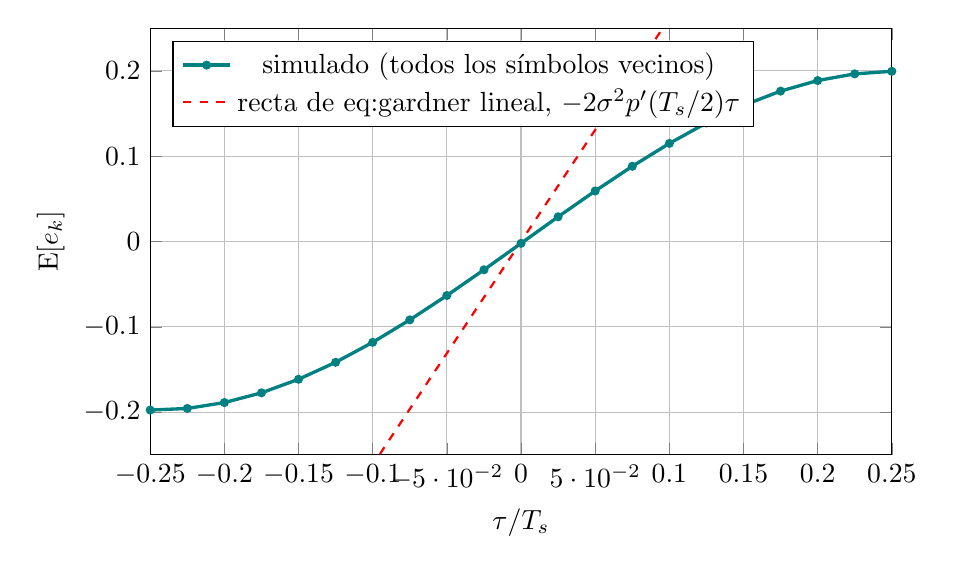
\begin{tikzpicture}
            \begin{axis}[
                width=11cm, height=7cm,
                xlabel={$\tau/T_s$},
                ylabel={$\mathrm E[e_k]$},
                xmin=-0.25, xmax=0.25,
                ymin=-0.25, ymax=0.25,
                grid=major,
                legend pos=north west,
                ]
                \addplot[teal, very thick, mark=*, mark size=1pt] coordinates {
                    (-0.250,-0.1975) (-0.225,-0.1956) (-0.200,-0.1887) (-0.175,-0.1773) (-0.150,-0.1614) (-0.125,-0.1415) (-0.100,-0.1181) (-0.075,-0.0918) (-0.050,-0.0632) (-0.025,-0.0331) (0.000,-0.0021) (0.025,0.0290) (0.050,0.0593) (0.075,0.0882) (0.100,0.1150) (0.125,0.1390) (0.150,0.1596) (0.175,0.1763) (0.200,0.1887) (0.225,0.1965) (0.250,0.1995)
                };
                \addlegendentry{simulado (todos los símbolos vecinos)}
                \addplot[Red, thick, dashed, domain=-0.25:0.25, samples=2] {2.617*x};
                \addlegendentry{recta de \eqref{eq:gardner lineal}, $-2\sigma^2p'(T_s/2)\tau$}
            \end{axis}
        \end{tikzpicture}
    \end{center}
    \caption{Señal de error de Gardner promediada, $\mathrm E[e_k]$, en función del error de temporización normalizado $\tau/T_s$, para un pulso de coseno alzado ($\alpha=0{,}35$) y símbolos $a_k=\pm 1$ (simulación con todos los símbolos vecinos, no solo los dos dominantes de la Proposición \ref{prop:gardner}). La curva es aproximadamente lineal y de signo correcto cerca de $\tau=0$, tal como predice \eqref{eq:gardner lineal} -- aunque, consistente con la Nota \ref{nota:gardner aproximacion}, la pendiente exacta difiere de la fórmula simplificada por el aporte de los símbolos más alejados.}\label{fig:gardner curva}
\end{figure}

\begin{remark}\label{nota:gardner aproximacion}
La Ecuación \eqref{eq:gardner lineal} retiene solo el aporte de los símbolos inmediatamente vecinos a cada muestra; un cálculo completo, incluyendo los símbolos más alejados que también contribuyen (el pulso de Nyquist no se anula \emph{estrictamente} fuera de $kT_s$ salvo en esos puntos), corrige la constante de proporcionalidad pero no cambia la conclusión cualitativa -- linealidad en $\tau$ y el signo del detector -- que es lo que importa para que el lazo enganche.
\end{remark}

\subsection*{Sincronización de trama}\label{sec:sincronizacion trama}

Con portadora y reloj de símbolo ya enganchados, el receptor recibe un flujo continuo y correctamente muestreado de símbolos -- pero sigue sin saber \emph{dónde}, dentro de ese flujo, empieza el mensaje que le interesa. Y, como vimos, puede no saber tampoco cuál de las rotaciones de fase ambiguas enganchó el lazo de portadora. Ambos problemas se resuelven con la misma herramienta: un \emph{preámbulo}, una secuencia de símbolos $s_0,\ldots,s_{L-1}$ \emph{conocida de antemano por transmisor y receptor}, transmitida al comienzo de cada trama.

El receptor busca el preámbulo \emph{correlacionando} la señal recibida contra la secuencia conocida, desplazando una ventana de longitud $L$ sobre el flujo de símbolos:
\begin{equation*}
    R[n] := \sum_{m=0}^{L-1} y_{n+m}\, s_m^*,
\end{equation*}
y evaluando $|R[n]|$ para cada posición candidata $n$. Si el preámbulo efectivamente empieza en $n=n_0$, entonces $y_{n_0+m}\approx s_m$ (a menos de ruido y, eventualmente, la rotación de fase ambigua) para $m=0,\ldots,L-1$, y $R[n_0]\approx\sum_m |s_m|^2$ -- la energía del preámbulo, un valor sustancialmente mayor que $R[n]$ para cualquier otro $n$, donde se están correlacionando símbolos de información (esencialmente aleatorios) contra la secuencia conocida. Buscar el máximo de $|R[n]|$ localiza entonces el inicio de la trama.

Para que este pico sea nítido -- y no se confunda con un máximo espurio en otra posición --, la secuencia $\{s_m\}$ debe diseñarse con \emph{buena autocorrelación}: un pico marcado en el desplazamiento nulo y valores chicos en cualquier otro desplazamiento. Existen familias de secuencias diseñadas explícitamente con este criterio; un ejemplo clásico son los \emph{códigos de Barker}, secuencias binarias ($s_m=\pm 1$) cuya autocorrelación fuera del pico principal está acotada por $1$ en valor absoluto. Por ejemplo, la secuencia de Barker de longitud $7$,
\begin{equation*}
    (s_0,\ldots,s_6) = (+1,+1,+1,-1,-1,+1,-1),
\end{equation*}
tiene autocorrelación $R[0]=7$ en el pico, y $|R[n]|\leqslant 1$ para todo $n\neq 0$ -- una relación pico a lóbulo de $7$ a $1$, excelente para una secuencia tan corta.

El preámbulo cumple, entonces, una doble función, que conecta directamente con lo desarrollado en esta sección:
\begin{itemize}
    \item \textbf{Marca el inicio de la trama}, vía el pico de correlación recién descripto.
    \item \textbf{Resuelve la ambigüedad de fase} (Sección \ref{sec:ambiguedad fase}): como el receptor conoce $s_m$, compara la fase del preámbulo \emph{recibido} contra la esperada y determina directamente cuál de las $m$ rotaciones ambiguas enganchó el lazo de Costas (o de decisión realimentada), corrigiéndola antes de decodificar el resto de la trama. De paso, al ser símbolos genuinamente conocidos (no decididos), es exactamente la secuencia de arranque que el lazo de decisión realimentada (Sección \ref{sec:decision directed}) necesitaba antes de poder confiar en sus propias decisiones.
\end{itemize}

Con esto se cierra el círculo de este capítulo: la ecualización le devuelve al pulso su forma libre de ISI (Sección \ref{sec:ecualizacion}), y el sincronismo de portadora, de símbolo y de trama garantizan, en conjunto, que el receptor demodula en la fase correcta, muestrea en el instante correcto, y sabe dónde empieza a leer -- las tres suposiciones que, desde el Capítulo \ref{chapter:deteccion ruido}, veníamos dando por sentado.




